\documentclass[11pt]{article}
\usepackage{acl}
\usepackage{times}
\usepackage{latexsym}
\usepackage[T1]{fontenc}
\usepackage[utf8]{inputenc}
\usepackage{microtype}
\usepackage{amsmath,amssymb}
\usepackage{graphicx}

\title{Giant Components under Random Failures: A Short Study from Single-Layer to Multilayer Networks}

\author{Chenhua Zhu \\
  Qinghai Normal University \\
  \texttt{zhu.chenhua@qq.com} \\
  \url{https://github.com/ZhuChenHua/study-multilayer-networks}}

\begin{document}
\maketitle

\begin{abstract}
  Understanding how networks remain connected under random failures is a central problem in network science. This short paper studies the basic concepts of connected components, the largest connected component, and the giant component under random attacks. We first review the generating-function formalism for single-layer networks and derive the classic ER (Erd\H{o}s--R\'enyi) result. We then move to multilayer interdependent networks, where the mutually connected giant component (MCGC) emerges through a discontinuous phase transition once two or more layers are present. Two small numerical experiments compare a single-layer ER network with a two-layer interdependent one, and then ask how the number of layers shifts the transition point. The complete simulation code is available online.
\end{abstract}

\section{Introduction}
Many real-world systems---power grids, the Internet, social platforms, and transportation networks---can be modeled as networks. A fundamental question is how robust these networks are when a fraction of nodes is randomly removed or fails. This process is often studied through percolation theory, where one asks whether a giant connected component still exists after random damage.

\begin{figure}[t]
  \centering
  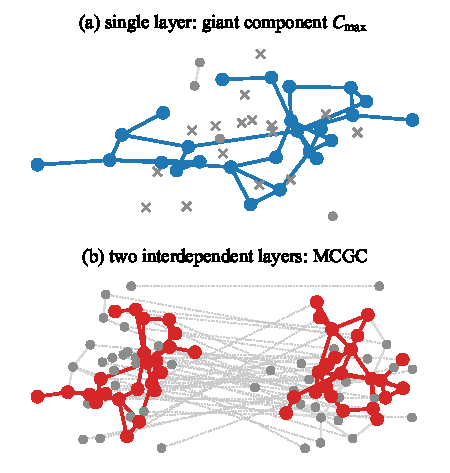
\includegraphics[width=\columnwidth]{figures/model.pdf}
  \caption{The two models studied here, for $N=45$, $c=4$ and $q=0.25$. (a) Single-layer ER network: after random removal only the largest connected component $C_{\max}$ (blue) matters. (b) Two interdependent ER layers: dotted lines connect replicas, and a node is in the mutually connected giant component (red) only if it lies in the giant component of both layers. Grey dots: other survivors; crosses: removed nodes.}
  \label{fig:model}
\end{figure}

In single-layer networks, the answer is relatively well understood. For random graphs and configuration models, generating functions give the size of the giant component and the percolation threshold~\cite{newman2010}. In multilayer networks~\cite{boccaletti2014}, however, the picture changes dramatically. When nodes in different layers depend on each other, a failure in one layer can trigger cascading failures in other layers, leading to a discontinuous collapse of the mutually connected giant component. Figure~\ref{fig:model} contrasts the two situations: in the single-layer case a node survives as soon as it stays connected, while in the interdependent case its replica must survive as well, and failures therefore propagate from one layer to the other until a mutually connected set remains.

This paper reviews percolation on networks from first principles: the core definitions, the main formulas, and two small numerical experiments. The full simulation code is available at \url{https://github.com/ZhuChenHua/study-multilayer-networks}.

\section{Definitions and Random Failure Model}
Let $G=(V,E)$ be an undirected graph with $N=|V|$ nodes. A \emph{connected component} is a maximal subset $C\subseteq V$ such that the induced subgraph $G[C]$ is connected. The \emph{largest connected component} is
\begin{equation}
  C_{\max} = \arg\max_{C\in \mathcal{C}(G)} |C|,
\end{equation}
where $\mathcal{C}(G)$ is the set of all connected components. If $|C_{\max}|$ scales linearly with $N$, it is called the \emph{giant component}.

In the random failure model, each node is removed independently with probability $q$. Equivalently, each node remains with probability $p=1-q$. After removal, we consider the induced subgraph on the remaining nodes. The quantity of interest is the ratio
\begin{equation}
  R(q) = \frac{|C_{\max}(G_q)|}{N},
\end{equation}
where $G_q$ is the remaining graph. We also write $S(q)$ for the same quantity when it is obtained from the generating-function formalism of Section~\ref{sec:single}; Section~\ref{sec:multi} reserves $S_{\mathrm{MCGC}}(q)$ for the multilayer case, so that the two are never confused.

\section{Single-Layer Percolation}\label{sec:single}
\subsection{Generating functions}
For a configuration-model network with degree distribution $P(k)$, define the generating functions
\begin{equation}
\begin{aligned}
  G_0(x)&=\sum_k P(k)x^k,\\
  G_1(x)&=\sum_k \frac{kP(k)}{\langle k\rangle}x^{k-1}.
\end{aligned}
\end{equation}
After random removal with probability $q$, let $u$ be the probability that a randomly chosen edge does not lead to the giant component. Then
\begin{equation}
  u = q + p G_1(u),
\end{equation}
and the giant component fraction is
\begin{equation}
  S = p[1-G_0(u)].
\end{equation}
The percolation threshold is determined by the first non-trivial solution of these equations~\cite{newman2010}.

\subsection{ER networks}
For an ER network~\cite{erdos1960} with average degree $c$, we have
\begin{equation}
  G_0(x)=G_1(x)=e^{-c(1-x)}.
\end{equation}
Thus the giant component fraction satisfies
\begin{equation}
  S = p(1-e^{-cS}) = (1-q)(1-e^{-cS}).
\end{equation}
The critical point is
\begin{equation}
  p_c = \frac{1}{c},\qquad q_c = 1-\frac{1}{c}.
\end{equation}
For $q<q_c$, a giant component exists; for $q>q_c$, it disappears.

\section{Multilayer Interdependent Networks}\label{sec:multi}
In a multiplex or interdependent network~\cite{buldyrev2010}, each node has a replica in every layer, and a node in one layer fails whenever its replica fails in another. The MCGC is the set of nodes that survive random removal and, in every layer, belong to one common connected cluster. It is obtained as the fixed point of an iteration: start from the survivors, and repeatedly replace the current set by the intersection, over all layers, of the largest connected component of that layer restricted to the current set. The iteration terminates when the set stops shrinking.

Consider $M$ layers, each an ER network with average degree $c$. After random removal with probability $q$, the MCGC fraction $S_{\mathrm{MCGC}}$ satisfies
\begin{equation}
\begin{aligned}
  S_{\mathrm{MCGC}} &= p(1-e^{-cS_{\mathrm{MCGC}}})^M\\
  &= (1-q)(1-e^{-cS_{\mathrm{MCGC}}})^M.
\end{aligned}
\end{equation}
This is the single-layer expression with one factor of $\bigl(1-e^{-cS}\bigr)$ per layer, the exponent $M$ counting the independent connectivity requirements. Formally it takes the same form as $S=p(1-G_0(u))$ of Section~\ref{sec:single} with $1-e^{-cS_{\mathrm{MCGC}}}$ in the role of $1-G_0(u)$ and the $M$ connectivity conditions raised to a power; the result is the size of the largest fixed point, which is the one selected by the iteration above. For $M=1$, this reduces to the single-layer ER result. For $M\ge 2$, the transition becomes discontinuous. The critical point is found by solving
\begin{equation}
  g_y(x)=x-y(1-e^{-x})^M=0,
  \qquad
  g_y'(x)=0,
\end{equation}
where $y=cp=c(1-q)$. Writing the first equation as $y=x/(1-e^{-x})^M$, the critical point is simply the maximum of this function,
\begin{equation}
  y_c = \max_{x>0} \frac{x}{(1-e^{-x})^M},
\end{equation}
whose maximizer satisfies $e^{x_c}=1+Mx_c$. For $M=1$ this gives $y_c=1$, i.e.\ $q_c=1-1/c$; for $M=2$ one obtains $x_c\approx 1.25643$ and $y_c\approx 2.45541$, so
\begin{equation}
  q_c = 1-\frac{y_c}{c}.
\end{equation}
This shows that interdependencies make the network more fragile: the transition is abrupt, and cascading failures can destroy the entire system. Since $y_c$ also grows with $M$, a system with more layers collapses at a smaller $q$.

\section{Numerical Experiments}
We perform two small simulations. In the first one we generate ER networks with $N=10{,}000$ nodes and average degree $c=4$. For the multilayer case, we generate two independent ER layers and couple each node with its replica in the other layer. We remove a fraction $q$ of nodes randomly, compute the largest connected component for the single-layer case and the MCGC for the two-layer case, and average over 20 independent runs.

Figure~\ref{fig:result} shows the results. The single-layer network exhibits a continuous transition near $q_c=0.75$, while the two-layer interdependent network collapses discontinuously at the smaller value $q_c=0.386$. The simulation points agree well with the theoretical curves obtained from the equations above.

\begin{figure}[t]
  \centering
  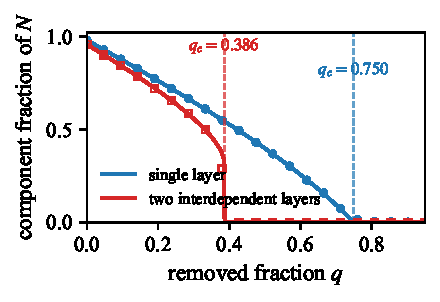
\includegraphics[width=\columnwidth]{figures/giant_component.pdf}
  \caption{Under random failures with $N=10{,}000$ and $c=4$: the single-layer quantity $R(q)=|C_{\max}|/N$ (blue) and the two-layer MCGC fraction $S_{\mathrm{MCGC}}$ (red), which are different quantities drawn on a common axis. Markers: simulation; lines: theory. The multilayer transition is discontinuous and occurs earlier.}
  \label{fig:result}
\end{figure}

The second simulation asks how the number of layers changes the transition. We generate $M=1,2,3,4$ interdependent ER layers with $N=4{,}000$ nodes and $c=6$, and average the MCGC fraction over 8 independent runs. Figure~\ref{fig:layers} shows that every curve with $M\ge 2$ jumps from zero at its own threshold, and that the threshold moves to smaller $q$ as $M$ grows ($q_c=0.833$, $0.591$, $0.485$ and $0.415$).

\begin{figure}[t]
  \centering
  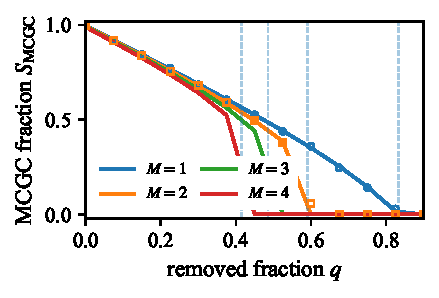
\includegraphics[width=\columnwidth]{figures/phase_transition.pdf}
  \caption{Effect of the number of layers, with $N=4{,}000$ and $c=6$, showing the MCGC fraction $S_{\mathrm{MCGC}}$. Markers: simulation; lines: theory; dashed lines: the thresholds $q_c=1-y_c/c$. The MCGC of $M\ge 2$ interdependent layers jumps from zero, at smaller $q$ as $M$ grows.}
  \label{fig:layers}
\end{figure}

\section{Conclusion and Code}
This paper studied the basics of random failures and giant components in single-layer and multilayer networks. The single-layer case is described by generating functions and the ER formula $S=(1-q)(1-e^{-cS})$. In multilayer interdependent networks, the MCGC follows $S_{\mathrm{MCGC}}=(1-q)(1-e^{-cS_{\mathrm{MCGC}}})^M$, and the transition becomes discontinuous for $M\ge 2$, with $y_c$ growing with $M$. The numerical experiments confirmed these predictions.

The complete simulation code, including network generation, random removal, BFS-based component detection, and plotting scripts, is available at
\begin{center}
  \url{https://github.com/ZhuChenHua/study-multilayer-networks}.
\end{center}
The model and the theory curves are implemented in \texttt{paper\_1/code/percolation.py}, and all three figures are produced by \texttt{paper\_1/code/figures.py}.

Both experiments point to the same open question: what happens when the layers are no longer identical, or when only a fraction $\alpha$ of the nodes depend on their replicas? Partial dependence does change the nature of the transition: coupling above a critical value gives the abrupt first-order collapse derived above, whereas reducing the coupling below that value turns the transition into a continuous one~\cite{parshani2010}. Extending the scripts to this regime would require adding the partial-dependence rule itself, since the current model assumes that every node depends on its replica in every layer.

\section*{Limitations}
The multilayer formula is derived for very large, simple networks, so for small networks it is slightly inaccurate near the threshold. We also assume that all layers are identical and that every node depends on its replica in every layer. The case where layers differ, or where only some nodes depend on their replicas, is not discussed here.

\bibliography{custom}

\appendix
\section{Formula and Symbol Reference}
The numbered equations and the symbols they use are collected here.

\paragraph{Equations.}
(1)~$C_{\max}=\arg\max_{C\in\mathcal C(G)}|C|$, the largest component; $\arg\max$ returns the component, not the size.
(2)~$R(q)=|C_{\max}(G_q)|/N$, the measured giant-component fraction after removing a fraction~$q$.
(3)~$G_0(x)=\sum_kP(k)x^k$ and $G_1(x)=\sum_k kP(k)x^{k-1}/\langle k\rangle$ are the node and edge generating functions.
(4)~$u=q+pG_1(u)$ is the self-consistency equation for the probability~$u$ that an edge does not lead to the giant component.
(5)~$S=p[1-G_0(u)]$ is the theoretical giant-component fraction.
(6)~$G_0(x)=G_1(x)=e^{-c(1-x)}$ for an ER network of mean degree~$c$.
(7)~$S=p(1-e^{-cS})=(1-q)(1-e^{-cS})$ is the single-layer ER equation; (8)~$p_c=1/c$ and $q_c=1-1/c$ are its critical points.
(9)~$S_{\mathrm{MCGC}}=p(1-e^{-cS_{\mathrm{MCGC}}})^M=(1-q)(1-e^{-cS_{\mathrm{MCGC}}})^M$ generalizes (7) to $M$ interdependent layers.
(10)~$g_y(x)=x-y(1-e^{-x})^M=0$ and $g_y'(x)=0$ determine the critical point, with $x=cS_{\mathrm{MCGC}}$ and $y=cp=c(1-q)$.
(11)~$y_c=\max_{x>0}x/(1-e^{-x})^M$ is the critical parameter; its maximizer satisfies $e^{x_c}=1+Mx_c$.
(12)~$q_c=1-y_c/c$ is the multilayer critical removal probability.

\paragraph{Symbols.}
$G=(V,E)$: undirected graph; $V$ nodes, $E$ edges; $N=|V|$: node count; $G[C]$: subgraph induced by~$C$; $C$: a connected component; $\mathcal C(G)$: set of all components; $C_{\max}$: largest component; $q$: removal probability; $p=1-q$: retention probability; $G_q$: remaining graph; $R(q)$: measured giant fraction; $S(q)$ and $S_{\mathrm{MCGC}}(q)$: theoretical giant fractions; $P(k)$: degree distribution; $k$: degree; $\langle k\rangle$: mean degree; $c$: ER mean degree; $G_0,G_1$: generating functions; $x$: their variable; $u$: probability an edge does not reach the giant component; $M$: number of layers; $y=cp$: rescaled control parameter; $g_y(x)$: auxiliary function; $x_c,y_c$: critical values; $p_c,q_c$: critical probabilities; $\alpha$: fraction of nodes depending on their replicas; $e$: base of the natural logarithm.

\end{document}